% abtex2-modelo-artigo.tex, v-1.9.2 laurocesar
% Copyright 2012-2014 by abnTeX2 group at http://abntex2.googlecode.com/ 
%

% ------------------------------------------------------------------------
% ------------------------------------------------------------------------
% abnTeX2: Modelo de Artigo Acadêmico em conformidade com
% ABNT NBR 6022:2003: Informação e documentação - Artigo em publicação 
% periódica científica impressa - Apresentação
% ------------------------------------------------------------------------
% ------------------------------------------------------------------------

\documentclass[
% -- opções da classe memoir --
article,			% indica que é um artigo acadêmico
11pt,				% tamanho da fonte
oneside,			% para impressão apenas no verso. Oposto a twoside
a4paper,			% tamanho do papel. 
% -- opções da classe abntex2 --
%chapter=TITLE,		% títulos de capítulos convertidos em letras maiúsculas
%section=TITLE,		% títulos de seções convertidos em letras maiúsculas
%subsection=TITLE,	% títulos de subseções convertidos em letras maiúsculas
%subsubsection=TITLE % títulos de subsubseções convertidos em letras maiúsculas
% -- opções do pacote babel --
english,			% idioma adicional para hifenização
brazil,				% o último idioma é o principal do documento
sumario=tradicional
]{abntex2}


% ---
% PACOTES
% ---

% ---
% Pacotes fundamentais 
% ---
\usepackage{lmodern}			% Usa a fonte Latin Modern
\usepackage[T1]{fontenc}		% Selecao de codigos de fonte.
\usepackage[utf8]{inputenc}		% Codificacao do documento (conversão automática dos acentos)
\usepackage{indentfirst}		% Indenta o primeiro parágrafo de cada seção.
\usepackage{nomencl} 			% Lista de simbolos
\usepackage{color}				% Controle das cores
\usepackage{graphicx}			% Inclusão de gráficos
\usepackage{float}
\usepackage{microtype} 			% para melhorias de justificação

% ---

% ---
% Pacotes adicionais, usados apenas no âmbito do Modelo Canônico do abnteX2
% ---
\usepackage{lipsum}				% para geração de dummy text
% ---

% ---
% Pacotes de citações
% ---
\usepackage[brazilian,hyperpageref]{backref}	 % Paginas com as citações na bibl
\usepackage[alf]{abntex2cite}	% Citações padrão ABNT
% ---

% ---
% Informações de dados para CAPA e FOLHA DE ROSTO
% ---
\titulo{Atividade IV }
\autor{ Rafael Gonçalves de Oliveira Viana}
\local{Brasil}
\data{2017}
% ---

% ---
% Configurações de aparência do PDF final

% alterando o aspecto da cor azul
\definecolor{blue}{RGB}{41,5,195}

% informações do PDF
\makeatletter
\hypersetup{
	%pagebackref=true,
	pdftitle={\@title}, 
	pdfauthor={\@author},
	pdfsubject={Artigo},
	pdfcreator={LaTeX with abnTeX2},
	pdfkeywords={abnt}{latex}{abntex}{abntex2}{atigo científico}, 
	colorlinks=true,       		% false: boxed links; true: colored links
	linkcolor=blue,          	% color of internal links
	citecolor=blue,        		% color of links to bibliography
	filecolor=magenta,      		% color of file links
	urlcolor=blue,
	bookmarksdepth=4
}
\makeatother
% --- 

% ---
% compila o indice
% ---
\makeindex
% ---

% ---
% Altera as margens padrões
% ---
\setlrmarginsandblock{3cm}{3cm}{*}
\setulmarginsandblock{3cm}{3cm}{*}
\checkandfixthelayout
% ---

% --- 
% Espaçamentos entre linhas e parágrafos 
% --- 

% O tamanho do parágrafo é dado por:
\setlength{\parindent}{1.3cm}

% Controle do espaçamento entre um parágrafo e outro:
\setlength{\parskip}{0.2cm}  % tente também \onelineskip

% Espaçamento simples
\SingleSpacing

% ----
% Início do documento
% ----
\begin{document}
	
	% Retira espaço extra obsoleto entre as frases.
	\frenchspacing 
	
	% ----------------------------------------------------------
	% ELEMENTOS PRÉ-TEXTUAIS
	% ----------------------------------------------------------
	
	%---
	%
	% Se desejar escrever o artigo em duas colunas, descomente a linha abaixo
	% e a linha com o texto ``FIM DE ARTIGO EM DUAS COLUNAS''.
	% \twocolumn[    		% INICIO DE ARTIGO EM DUAS COLUNAS
	%
	%---
	% página de titulo
	\maketitle
	\begin{enumerate}
		\item Inserir 10 Instrutores.
				\begin{verbatim}
				insert into instrutores (cod_instrutor, nome_instrutor, tel_instrutor, admissao) 
				values (71, 'Felipe', '223-139', to_date('1/2/2017','dd/mm/yyyy'));
				
				insert into instrutores (cod_instrutor, nome_instrutor, tel_instrutor, admissao) 
				values (72, 'Carlos', '132-339', to_date('2/3/2017','dd/mm/yyyy'));
				
				insert into instrutores (cod_instrutor, nome_instrutor, tel_instrutor, admissao) 
				values (73, 'Luiz', '173-839', to_date('4/3/2017','dd/mm/yyyy'));
				
				insert into instrutores (cod_instrutor, nome_instrutor, tel_instrutor, admissao) 
				values (74, 'Thiago', '273-919', to_date('12/3/2017','dd/mm/yyyy'));
				
				insert into instrutores (cod_instrutor, nome_instrutor, tel_instrutor, admissao) 
				values (75, 'Pablo', '423-229', to_date('3/4/2017','dd/mm/yyyy'));
				
				insert into instrutores (cod_instrutor, nome_instrutor, tel_instrutor, admissao) 
				values (76, 'Juana', '173-291', to_date('4/4/2017','dd/mm/yyyy'));
				
				insert into instrutores (cod_instrutor, nome_instrutor, tel_instrutor, admissao) 
				values (77, 'Luana', '243-419', to_date('22/4/2017','dd/mm/yyyy'));
				
				insert into instrutores (cod_instrutor, nome_instrutor, tel_instrutor, admissao) 
				values (78, 'Rafaela', '13-229', to_date('3/5/2017','dd/mm/yyyy'));
				
				insert into instrutores (cod_instrutor, nome_instrutor, tel_instrutor, admissao) 
				values (79, 'Daniela', '273-519', to_date('23/5/2017','dd/mm/yyyy'));
				
				insert into instrutores (cod_instrutor, nome_instrutor, tel_instrutor, admissao) 
				values (80, 'Tommyy', '221-239', to_date('25/5/2017','dd/mm/yyyy'));
				
				insert into instrutores (cod_instrutor, nome_instrutor, tel_instrutor, admissao) 
				values (81, 'Dany', '221-239', to_date('26/5/2017','dd/mm/yyyy'));​
				
				\end{verbatim}
				\vspace{0.5cm}
				\begin{center}
					\begin{figure}[H]
						\centering
						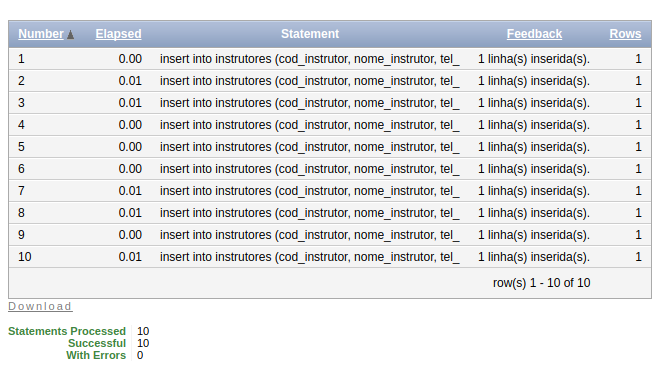
\includegraphics[scale=0.5]{./at-01.png}
						\caption{Inicio de sondagem com um hospedeiro alvo.}
						\label{rota-1}
					\end{figure}
				\end{center}
			
			
			\item Inserir 10 Cursos.
			\begin{verbatim}
			
			insert into cursos (cod_curso, nome_curso, carga_horaria , preco, pre_requisito)
			values (30, 'Mecânica', 32, 200, 1);
			
			insert into cursos (cod_curso, nome_curso, carga_horaria , preco, pre_requisito)
			values (31, 'Robótica Avançada', 34, 250, 2);
			
			insert into cursos (cod_curso, nome_curso, carga_horaria , preco, pre_requisito)
			values (32, 'Warms', 19, 40, 2);
			
			insert into cursos (cod_curso, nome_curso, carga_horaria , preco, pre_requisito)
			values (33, 'DoS', 22, 150, 6);
			
			insert into cursos (cod_curso, nome_curso, carga_horaria , preco, pre_requisito)
			values (34, 'Mongoose', 22, 980, 2);
			
			insert into cursos (cod_curso, nome_curso, carga_horaria , preco, pre_requisito)
			values (35, 'Mongo', 68, 400, 6);
			
			insert into cursos (cod_curso, nome_curso, carga_horaria , preco, pre_requisito)
			values (36, 'Express', 32, 400, 1);
			
			insert into cursos (cod_curso, nome_curso, carga_horaria , preco, pre_requisito)
			values (37, 'Node ', 32, 250, 5);
			
			insert into cursos (cod_curso, nome_curso, carga_horaria , preco, pre_requisito)
			values (38, 'Angular 4', 24, 150, 4);
			
			insert into cursos (cod_curso, nome_curso, carga_horaria , preco, pre_requisito)
			values (39, 'Angular 2', 3, 100, 1);
			
			insert into cursos (cod_curso, nome_curso, carga_horaria , preco, pre_requisito)
			values (40, 'Redes III', 3, 200, 7);​
		
			\end{verbatim}
			\vspace{0.4cm}
			\begin{center}
				\begin{figure}[H]
					\centering
					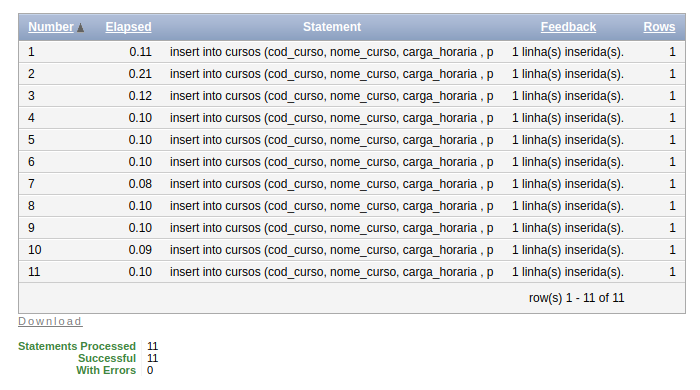
\includegraphics[scale=0.5]{./at-02.png}
					\caption{Inicio de sondagem com um hospedeiro alvo.}
					\label{rota-1}
				\end{figure}
			\end{center}
			
		\item Inserir 10 Alunos.
			
				\begin{verbatim}
					insert into alunos 
					(matricula, nome_aluno, tel_aluno, endereco_aluno, cidade_aluno, uf)
					values 
					(81, 'Pedro S Joao', '347-2318', 'Rua das Flores, 222', 'São Pedro', 'SP');
					
					insert into alunos 
					(matricula, nome_aluno, tel_aluno, endereco_aluno, cidade_aluno, uf)
					values
					(82, 'Tommy F Paulo ', '399-1490', 'R. Albert Einstein, 102', 'Campinas', 'MG');
					
					insert into alunos 
					(matricula, nome_aluno, tel_aluno, endereco_aluno, cidade_aluno, uf)
					values
					(83, 'Tomaz A Turbano', '115-1138', 'Av. Pedro, 50', 'Linhares', 'SP');
					
					insert into alunos 
					(matricula, nome_aluno, tel_aluno, endereco_aluno, cidade_aluno, uf)
					values 
					(84, 'Jota A Jota', '331-1171', 'Av. Tomy, Casa 2', 'Barbacena', 'MG');
					
					insert into alunos
					(matricula, nome_aluno, tel_aluno, endereco_aluno, cidade_aluno, uf)
					values 
					(85, 'Pedro F Paulo', '111-2122', 'Av. 15 de Abril, 3502', 'Sorocaba', 'SP');
					
					insert into alunos
					 (matricula, nome_aluno, tel_aluno, endereco_aluno, cidade_aluno, uf)
					values 
					(86, 'Julio Q Pedro', '961-5442', 'Av. Tieta, 17/12', 'Sao Paulo', 'SP');
					
					insert into alunos
					 (matricula, nome_aluno, tel_aluno, endereco_aluno, cidade_aluno, uf)
					values
					 (87, 'Joao P Lucas', '112-5322', 'Av. dos Limoeiros, 42', 'Belo Horizonte', 'MG');
					
					insert into alunos 
					(matricula, nome_aluno, tel_aluno, endereco_aluno, cidade_aluno, uf)
					values
					 (88, 'Jota S Luiz', '113-3323', 'R. Silva, 326', 'Campos', 'SP');
					
					insert into alunos
					(matricula, nome_aluno, tel_aluno, endereco_aluno, cidade_aluno, uf)
					values 
					(89, 'Reis ACarlos', '441-6120', 'R. Pedro Luis, 112', 'Uberaba', 'MG');
					
					insert into alunos 
					(matricula, nome_aluno,tel_aluno, endereco_aluno, cidade_aluno, uf)
					 values 
					(90, 'Marceu de Pedro', '121-1339', 'R. Joaquim Hernandez, 1/703', 'Vitoria', 'ES');
					
				\end{verbatim}
			\vspace{0.3cm}
			\begin{center}
				\begin{figure}[H]
					\centering
					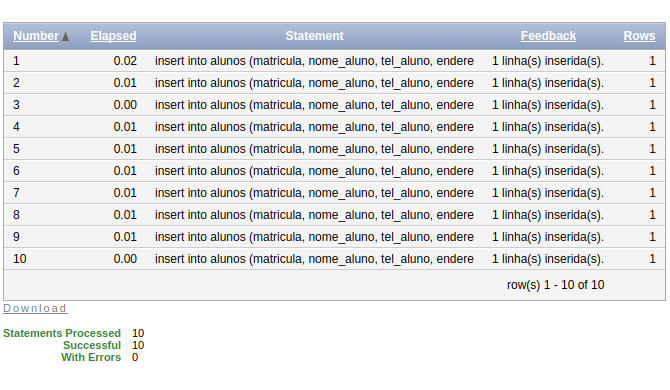
\includegraphics[scale=0.5]{./at-03.png}
					\caption{Inicio de sondagem com um hospedeiro alvo.}
					\label{rota-1}
				\end{figure}
			\end{center}

			\item Inserir 5 Turmas.
		
		\begin{verbatim}
			insert into turmas (cod_turma, cod_curso, cod_instrutor, preco_hora_instrutor, sala) 
			values (59, 34, 73, 12, 4);
			
			insert into turmas (cod_turma, cod_curso, cod_instrutor, preco_hora_instrutor, sala) 
			values (60, 34, 72, 16, 1);
			
			insert into turmas (cod_turma, cod_curso, cod_instrutor, preco_hora_instrutor, sala) 
			values (61, 34, 74, 14, 3);
			
			insert into turmas (cod_turma, cod_curso, cod_instrutor, preco_hora_instrutor, sala) 
			values (62, 34, 75, 10, 6);
			
			insert into turmas (cod_turma, cod_curso, cod_instrutor, preco_hora_instrutor, sala) 
			values (63, 35, 76, 22, 7);
		\end{verbatim}
		\begin{center}
			\begin{figure}[H]
				\centering
				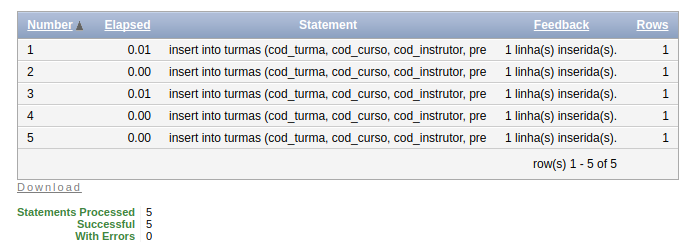
\includegraphics[scale=0.5]{./at-04.png}
				\caption{Inicio de sondagem com um hospedeiro alvo.}
				\label{rota-1}
			\end{figure}
		\end{center}
			\item Inserir 15 Historicos.
		
		\begin{verbatim}
		insert into historico (cod_turma, matricula, nota)
		values (59, 21, 8.5);
		
		insert into historico (cod_turma, matricula, nota)
		values (59, 22, 9.5);
		
		insert into historico (cod_turma, matricula, nota)
		values (60, 23, 7.5);
		
		insert into historico (cod_turma, matricula, nota)
		values (61, 23, 8.5);
		
		insert into historico (cod_turma, matricula, nota)
		values (62, 24, 10);
		
		insert into historico (cod_turma, matricula, nota)
		values (63, 25, 2);
		
		insert into historico (cod_turma, matricula, nota)
		values (63, 26, 4);
		
		insert into historico (cod_turma, matricula, nota)
		values (63, 27, 7);
		
		insert into historico (cod_turma, matricula, nota)
		values (62, 28, 2.5);
		
		insert into historico (cod_turma, matricula, nota)
		values (62, 29, 1.5);
		
		insert into historico (cod_turma, matricula, nota)
		values (60, 30, 4.5);
		
		insert into historico (cod_turma, matricula, nota)
		values (61, 31, 9.5);
		
		insert into historico (cod_turma, matricula, nota)
		values (60, 32, 10);
		
		insert into historico (cod_turma, matricula, nota)
		values (62, 33, 7.5);
		
		insert into historico (cod_turma, matricula, nota)
		values (63, 34, 9.5);​
		​
		\end{verbatim}
		\vspace{0.0cm}
		\begin{center}
			\begin{figure}[H]
				\centering
				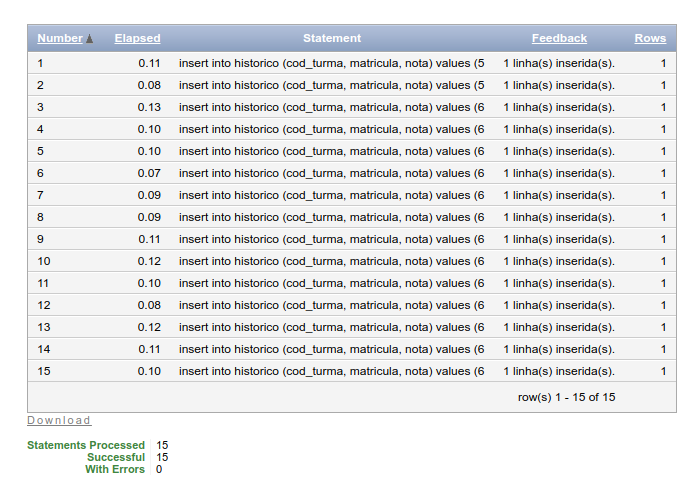
\includegraphics[scale=0.5]{./at-05.png}
				\caption{Inicio de sondagem com um hospedeiro alvo.}
				\label{rota-1}
			\end{figure}
		\end{center}
\end{enumerate}
	
		
	\section{Buscas}
	 
	 \begin{enumerate}
	 	\item  Recuperar o nome e endereço dos alunos que
	 	são do estado do Rio de Janeiro (uf = 'RJ').
	 	\begin{verbatim}
	 		
	 		select nome_aluno, endereco_aluno from alunos where uf='RJ';
	 	\end{verbatim}
	 		\begin{center}
	 		\begin{figure}[H]
	 			\centering
	 			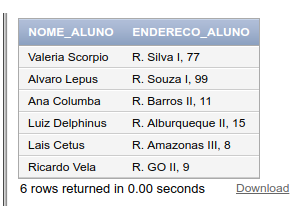
\includegraphics[scale=0.5]{./at-06.png}
	 			\caption{Inicio de sondagem com um hospedeiro alvo.}
	 			\label{rota-1}
	 		\end{figure}
	 	\end{center}
	 	
	 	\item  Recuperar o nome de todos os instrutores e a
	 	data de admissão.
	 	\begin{verbatim}
		     	select nome_instrutor, admissao from instrutores;
	 	\end{verbatim}
	 	\begin{center}
	 		\begin{figure}[H]
	 			\centering
	 			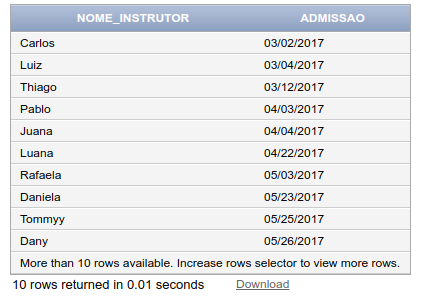
\includegraphics[scale=0.5]{./at-07.png}
	 			\caption{Inicio de sondagem com um hospedeiro alvo.}
	 			\label{rota-1}
	 		\end{figure}
	 	\end{center}
	 	
	 	
	 	 	
	 	\item  Recuperar o nome do curso e o cod\_turma de
	 	cada turma.
	 	\begin{verbatim}
select c.nome_curso,t.cod_turma from turmas t, cursos c where
 t.cod_curso=c.cod_curso;
	 	\end{verbatim}
	 	\begin{center}
	 		\begin{figure}[H]
	 			\centering
	 			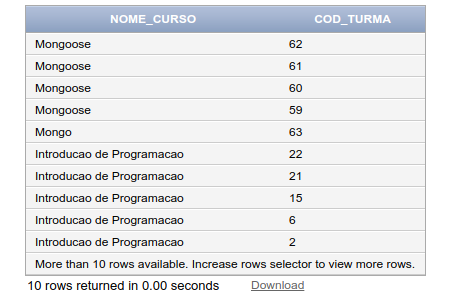
\includegraphics[scale=0.5]{./at-08.png}
	 			\caption{Inicio de sondagem com um hospedeiro alvo.}
	 			\label{rota-1}
	 		\end{figure}
	 	\end{center}
	 	
	 	
	 	\item  Recuperar o nome e o telefone dos instrutores
	 	de 'Fundamentos da Modelagem de Dados'.
	 	\begin{verbatim}
	 	select c.nome_curso,t.cod_turma from turmas t, cursos c where
	 	t.cod_curso=c.cod_curso;
	 	\end{verbatim}
	 	\begin{center}
	 		\begin{figure}[H]
	 			\centering
	 			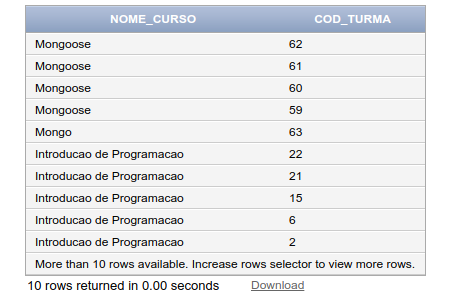
\includegraphics[scale=0.5]{./at-08.png}
	 			\caption{Inicio de sondagem com um hospedeiro alvo.}
	 			\label{rota-1}
	 		\end{figure}
	 	\end{center}
	 		\item  Recuperar o nome do aluno, sua nota e o nome
	 		do instrutor, do curso de 'Redes I'.
	 	\begin{verbatim}
	 	select c.nome_curso,t.cod_turma from turmas t, cursos c where
	 	t.cod_curso=c.cod_curso;
	 	\end{verbatim}
	 	\begin{center}
	 		\begin{figure}[H]
	 			\centering
	 			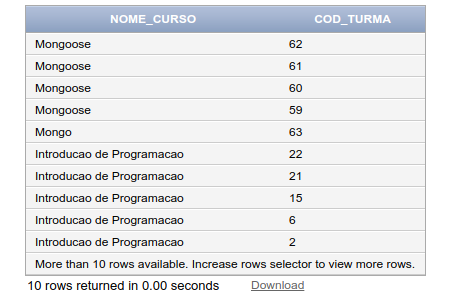
\includegraphics[scale=0.5]{./at-08.png}
	 			\caption{Inicio de sondagem com um hospedeiro alvo.}
	 			\label{rota-1}
	 		\end{figure}
	 	\end{center}
	 	
	 	
 	\end{enumerate}
	 	


	
	
\end{document}